\scanpage{78}
% archive foliation: 77
\figure{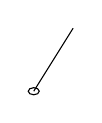
\begin{tikzpicture}[x=1mm,y=1mm]\draw (0,0) ellipse(.7mm and .45mm);\draw (0,0)--(5,8);\end{tikzpicture}}
$H^2(S,A)\deleted{\unsure{\otimes\mathbf{Q}_\ell}}$ (dont le $T_\ell$ est $H^2(S,T_\ell(A))$) n'est pas néc nul, \deleted{\unsure{si}} \inserted{comme on voit} si $S$ est une courbe lisse projective géom. connexe sur $\mathbf{F}_p$ et $A=J\times S$, où $J$ est la jacobienne de $S$.
On a en tous cas
\[
\begin{aligned}
H^2(S,T_\ell(A))&\simeq H^1(\overline{S},T_\ell(\overline{A}))_\pi\\
&=\deleted{T_\ell J(\overline{\mathbf{F}}_p)\otimes}\inserted{[T_\ell(\unsure{\check{J}|\overline{J}})\otimes T_\ell(\overline{J})]_\pi}\\
&\simeq\mathrm{End}(J)\otimes_{\unsure{\mathbf{Z}|\mathbf{Q}}}\mathbf{Q}_\ell\quad\deleted{\unsure{par}}\ (\simeq(\unsure{\text{bihom}|\text{classes}}\text{ de corr. }\inserted{\text{divisorielles}}\text{ sur }C\,C)\otimes_{\mathbf{Z}}\mathbf{Q}_\ell
\end{aligned}
\]
qui est non nul .....
